\section{Техническое задание}
\subsection{Основание для разработки}

Основанием для разработки является задание на выпускную квалификационную работу бакалавра "<Программно-информационная система создания 2D-изображений и их интерактивной визуализации">.

\subsection{Цель и назначение разработки}

Целью данной выпускной квалификационной работы является создание программно-информационной системы, позволяющей автоматически генерировать карты нормалей из 2D-изображений и визуализировать результат в интерактивной форме с возможностью настройки освещения и параметров генерации.

Основной задачей разработки является не только получение карты нормалей, но и наглядная демонстрация, как такие карты влияют на восприятие текстуры при освещении, что особенно важно при создании графики для видеоигр и 3D-приложений \cite{matiz2020}.

Разрабатываемая программа решает следующие задачи:
\begin{enumerate}
	\item Преобразование 2D-изображений в карты нормалей с помощью операторов градиентов (например, оператора Собеля).
	\item Поддержка различных параметров генерации карт нормалей (интенсивность, гладскость, инвертирование, выбор метода).
	\item Загрузка и сохранение изображений и карт нормалей в удобных графических форматах.
	\item Отображение результата с реалистичным эффектом освещения от виртуального источника света ("фонарика").
	\item Настройка параметров визуализации (интенсивность света, радиус, положение источника).
	\item Интерактивное управление освещением с помощью пользовательского ввода (например, движения мыши).
	\item Просмотр освещенной текстуры в 2D и 3D режимах.
	\item Обеспечение простого графического интерфейса, соответствующего макету и требованиям пользовательского опыта.
\end{enumerate}
\subsection{Требования к программной системе}

Данный раздел определяет перечень требований, которым должна соответствовать разрабатываемая программно-информационная система. Требования подразделяются на функциональные, нефункциональные, интерфейсные, а также программно-аппаратные. Эти требования служат основой для реализации, тестирования и оценки готовности программного продукта \cite{johnson2020}.
\subsubsection{Функциональные требования}

Программа должна обеспечивать выполнение следующих функций:
\begin{enumerate}
	\item Загрузка изображения с поддержкой форматов PNG, JPEG, BMP и отображением загруженного изображения в интерфейсе.
	\item Генерация карты нормалей с применением одного из выбранных операторов градиента: Sobel, Prewitt, Scharr, возможность управлять этими параметрами.
	\item Отображение исходного изображения и соответствующей ему карты нормалей, возможность изменения параметров генерации с обновлением результата.
	\item Наложение карты нормалей на исходную текстуру с учетом освещения, настройка интенсивности и радиуса света.
	\item Сохранение сгенерированной карты нормалей в файл.
	\item Наложение карты нормалей (в 2D-режиме) на изображение с имитацией освещения (эффект фонарика), настройка интенсивности, радиуса и фонового освещения.
	\item Отображение изображения (в 3D-режиме) на гранях вращающегося куба с освещением на основе нормалей и камеры пользователя.
	\item Переключение между режимами визуализации (2D и 3D) в реальном времени без потери данных и с сохранением текущих параметров генерации.
	\item Настройка всех вышеуказанных параметров через GUI в реальном времени.
\end{enumerate}
\subsubsection{Нефункциональные требования}

Программа должна соответствовать следующим нефункциональным требованиям:
\begin{enumerate}
	\item Удобство использования. Интерфейс должен быть интуитивно понятным и доступным пользователю без необходимости изучения технической документации.
	\item Производительность. Обработка изображений до 4096×4096 пикселей не должна занимать более нескольких секунд на стандартном ПК.
	\item Надёжность. Обработка ошибок (например, при загрузке неподдерживаемого формата).
	\item Наложение карты нормалей на исходную текстуру с учетом освещения, настройка интенсивности и радиуса света.
	\item Масштабируемость. Возможность расширения функциональности в будущем (например, добавление новых операторов, поддержку глубинных карт и др.).
\end{enumerate}
\paragraph{Интерфейсные требования}

Основное окно приложения должно включать:
\begin{itemize}
	\item панель для исходного изображения;
	\item панель для сгенерированной карты нормалей;
	\item элементы управления параметрами генериции нормалей;
	\item элементы управления параметрами освещения (интенсивность, радиус и пр.);
	\item кнопки загрузки и сохранения;
	\item панель для визулизации;
	\item выпадающий список с выбором оператора;
	\item выпадающий список с выбором режима (2D и 3D);
	\item чекбокс для инвертирования нормали.
\end{itemize}

Визуальная структура и выравнивание:
\begin{itemize}
	\item расположение всех элементов интерфейса должно соответствовать макету;
	\item кнопка сохранения расположена под с окном "Карта нормалей";
	\item кнопка загрузки расположена под с окном "Исходное изображение";
	\item блок "параметры нормалей" включает: силу, глубину, выбор оператора, выбор режима и инвертирование;
	\item блок "параметры освещения" включает в себя: яркость окружения, радиус и силу "фонарика".
\end{itemize}

Все изменения параметров происходят в реальном времени.

Макет приложения представлен на рисунке ~\ref{mak2:image}.

\begin{figure}[ht]
	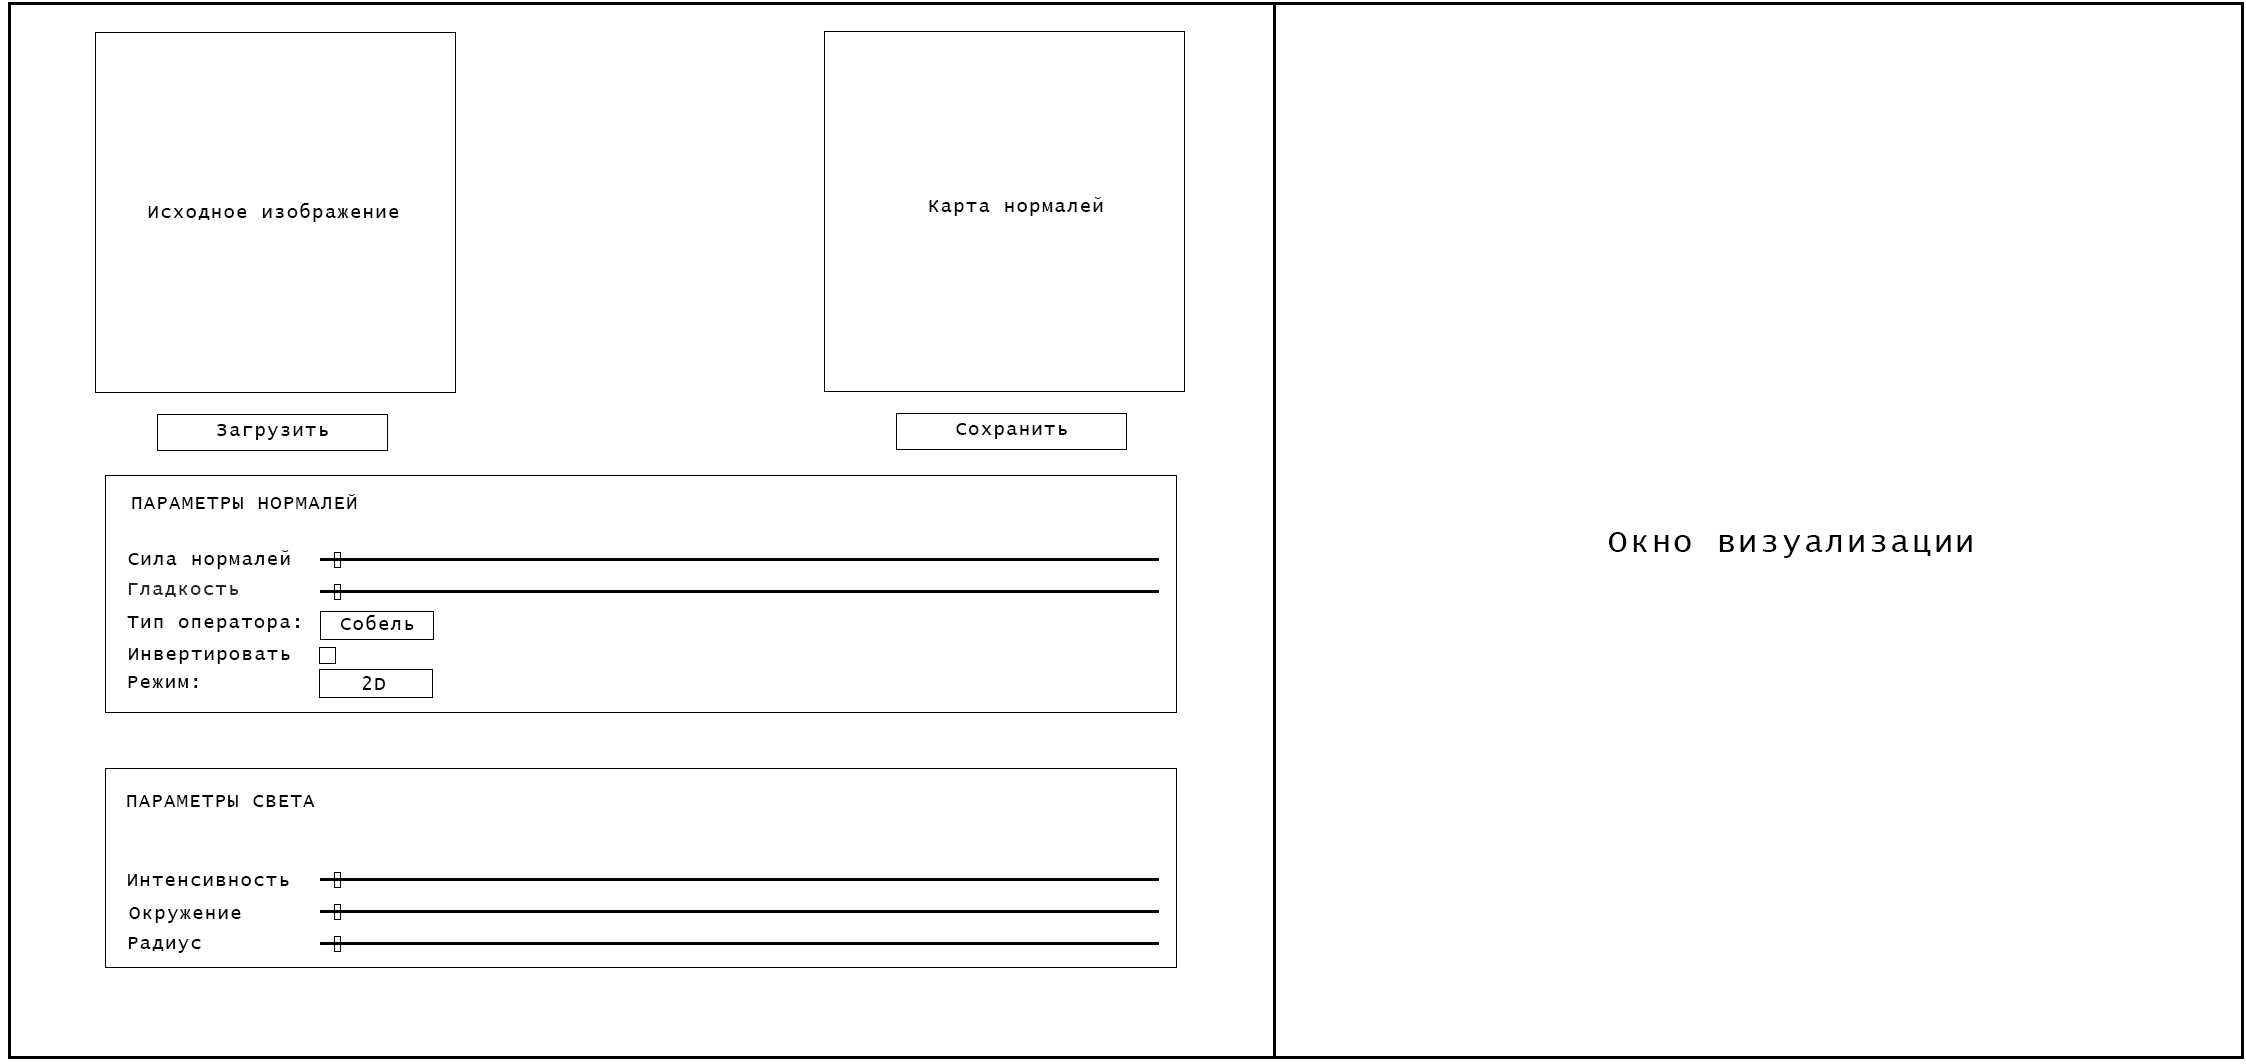
\includegraphics[width=1\linewidth]{mak2}
	\caption{Макет приложения}
	\label{mak2:image}
\end{figure}
\paragraph{Программные требования}

Для реализации программной информационной системы генерации карт нормалей из 2D-изображений и их визуализации используется язык программирования Python версии не ниже 3.10. Данный язык был выбран ввиду его гибкости, широкого набора библиотек для обработки изображений и создания графических интерфейсов, а также активного сообщества \cite{ramalho2022}.

При разработке используются следующие библиотеки и инструменты:
\begin{enumerate}
	\item PyQt5 — для построения графического интерфейса пользователя.
	\item OpenCV — для обработки изображений, включая применение операторов градиента (Sobel, Scharr, Prewitt).
	\item NumPy — для численных операций и работы с массивами данных.
	\item Pillow (PIL) — для загрузки и сохранения изображений.
	\item PyOpenGL — обёртка над OpenGL, используемая для реализации 3D-визуализации: отрисовки куба, применения текстур, настройки источника света, обработки взаимодействия с мышью и колесом прокрутки.
	\item math — стандартный модуль Python, применяемый для математических вычислений в процессе нормализации векторов и построения 3D-сцены.
\end{enumerate}

Программа является десктопным приложением и предназначена для запуска на операционных системах Windows 10/11.

Минимальные версии компонентов:
\begin{itemize}
	\item Python 3.10+;
	\item OpenCV 4.5+;
	\item PyQt5 5.15+;
	\item NumPy 1.21+;
	\item Pillow (PIL) 8.0+;
	\item PyOpenGL 3.1+.
\end{itemize}
\paragraph{Аппаратные требования}

Для корректной работы программной системы требуется следующее минимальное аппаратное обеспечение:
\begin{enumerate}
	\item Центральный процессор: 4-ядерный с частотой не ниже 2.0 ГГц (рекомендуется ≥ 6 ядер).
	\item Оперативная память: минимум 8 ГБ (рекомендуется ≥ 16 ГБ для работы с большими изображениями).
	\item Графический процессор (опционально): для ускорения визуализации возможно использование GPU с поддержкой OpenGL 3.3 и выше.
	\item Жесткий диск: не менее 500 МБ свободного пространства для установки и хранения изображений.
	\item Разрешение экрана: минимум 1280×720 пикселей (рекомендуется 1920×1080 и выше).
	\item Операционная система: Windows 10/11.
\end{enumerate}

Наличие подключения к интернету не является обязательным для работы программы, но может использоваться при обновлениях или загрузке дополнительных изображений с онлайн-источников.
\paragraph{Требования к надёжности}

Разрабатываемое приложение представляет собой десктопную программу, работающую в автономном режиме без необходимости постоянного подключения к сети Интернет. Однако, несмотря на это, могут возникать ситуации, при которых необходима высокая устойчивость и корректное поведение приложения.

Возможные непредвиденные ситуации при работе программы:
\begin{enumerate}
	\item Преждевременное завершение работы из-за аварийного завершения ОС (например, выключение ПК, перезагрузка).
	\item Некорректное изображение или файл, не соответствующий ожидаемому формату.
	\item Отсутствие доступа к диску (например, при попытке сохранить файл на недоступный путь).
	\item Ошибки при работе с внешними библиотеками или повреждёнными изображениями.
\end{enumerate}

Меры повышения надёжности:
\begin{enumerate}
	\item Обработка всех исключений, связанных с загрузкой, сохранением и визуализацией изображений.
	\item Проверка корректности форматов данных до начала обработки.
	\item Автоматическое уведомление пользователя об ошибке с понятным описанием причины.
\end{enumerate}
\paragraph{Требования к оформлению документации}

Требования к стадиям разработки программ и программной документации для вычислительных машин, комплексов и систем независимо от их назначения и области применения, этапам и содержанию работ устанавливаются ГОСТ 19.102–77.

Программная документация должна включать в себя:
\begin{enumerate}
	\item Анализ предметной области.
	\item Техническое задание.
	\item Технический проект.
	\item Рабочий проект.	
\end{enumerate}
\subsection{Входные и выходные данные}

Данный раздел описывает, с какими данными работает разрабатываемая программно-информационная система на входе и выходе. Это необходимо для понимания характера обрабатываемой информации, форматов файлов и способов интерпретации результатов пользователем \cite{dawson2021}.
\subsubsection{Входные данные}

Входными данными для программного продукта являются:
\begin{enumerate}
	\item 2D-изображение (текстура). Пользователь может загрузить произвольное изображение, которое будет использоваться для генерации карты нормалей. Поддерживаются следующие форматы:
	\begin{itemize}
		\item PNG (.png);
		\item JPEG (.jpg, .jpeg).
	\end{itemize}
	\item Параметры генерации нормалей, устанавливаемые через пользовательский интерфейс:
	\begin{itemize}
		\item оператор градиента: выбор между Sobel, Scharr, Prewitt;
		\item сила нормалей (амплитуда влияния градиента);
		\item гладкость нормалей (масштаб Z-компоненты);
		\item инверсия нормалей (по оси X, Y, Z);
		\item выбор режима (2D, 3D).
	\end{itemize}	
	\item Параметры визуализации:
	\begin{itemize}
		\item интенсивность света (яркость источника);
		\item радиус фонарика (область действия);
		\item свет окружения;
		\item положение источника света (движение мышью в интерактивном режиме).
	\end{itemize}	
\end{enumerate}

Все параметры могут быть изменены пользователем до или после загрузки изображения. Программа немедленно пересчитывает результат при изменении параметров.
\subsubsection{Выходные данные}

Выходные данные делятся на основные (результаты генерации) и вспомогательные (визуализация, сохранение):
\begin{enumerate}
	\item Карта нормалей представлена в виде цветного изображения, где:
	\begin{itemize}
		\item формат файла: PNG (бессжатый);
		\item цветовое пространство — стандартное RGB;
	\end{itemize}	
	\item Визуализированная текстура с освещением:
	\begin{itemize}
		\item представляет собой наложение карты нормалей на исходную текстуру с учётом виртуального освещения;
		\item реализация через симуляцию источника света, перемещаемого мышью (в 2D);
		\item выходной формат: PNG.
	\end{itemize}	
\end{enumerate}
\subsection{Варианты использования}

Диаграмма прецендентов представлена на рисунке ~\ref{prec3:image}.

\begin{figure}[ht]
	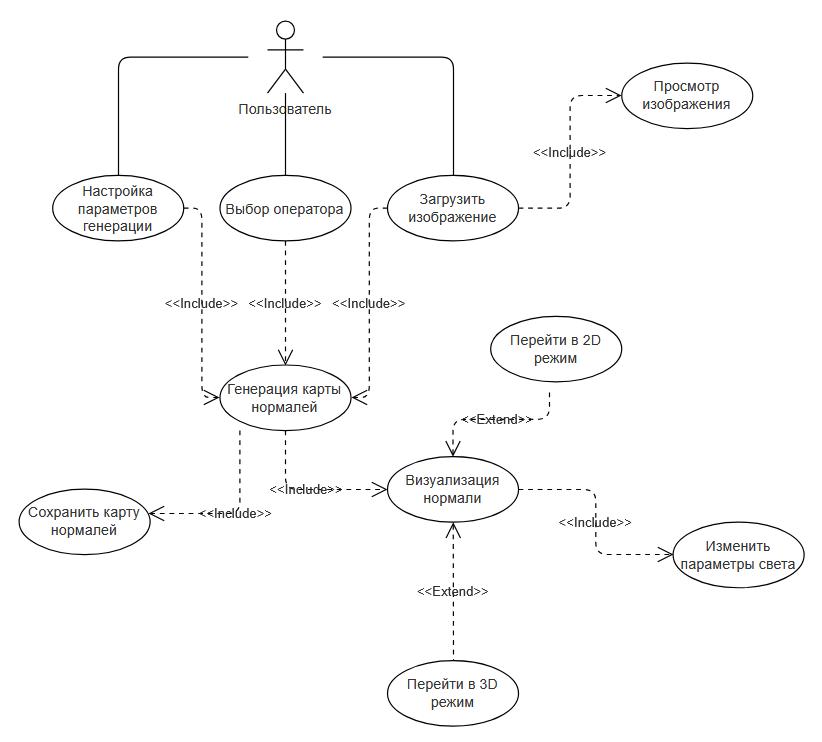
\includegraphics[width=1\linewidth]{prec3}
	\caption{Диаграмма прецендентов}
	\label{prec3:image}
\end{figure}
\subsubsection{Вариант использования «Загрузка изображения»}

Заинтересованные лица и их требования: пользователь хочет загрузить своё изображение (например, текстуру) в приложение, чтобы сгенерировать карту нормалей.

Предусловие: приложение запущено. Пользователь находится на вкладке генерации.

Постусловие: изображение отображается в левой части интерфейса, готовое к дальнейшей обработке.

Основной успешный сценарий:
\begin{enumerate}
	\item Пользователь нажимает кнопку «Загрузить».
	\item Система открывает диалог выбора файла.
	\item Пользователь выбирает изображение в поддерживаемом формате (PNG, JPG и др.).
	\item Система загружает изображение и отображает его на панели.
\end{enumerate}
\subsubsection{Вариант использования «Сохранение карты нормалей»}

Заинтересованные лица и их требования: пользователь хочет сохранить сгенерированную карту нормалей для дальнейшего использования.

Предусловие: карта нормалей сгенерирована и отображена в правой панели.

Постусловие: изображение с картой нормалей сохранено в выбранную папку.

Основной успешный сценарий:
\begin{enumerate}
	\item Пользователь нажимает кнопку «Сохранить».
	\item Открывается диалог выбора пути сохранения.
	\item Пользователь указывает имя файла и формат (PNG).
	\item Система сохраняет изображение.
\end{enumerate}
\subsubsection{Вариант использования «Визуализация освещения в 2D»}

Заинтересованные лица и их требования: пользователь хочет оценить, как карта нормалей влияет на освещение в 2D-режиме.

Предусловие: карта нормалей сгенерирована, выбран режим 2D.

Постусловие: система отображает наложенное освещение с учётом перемещаемого источника света.

Основной успешный сценарий:
\begin{enumerate}
	\item Пользователь наводит курсор на область изображения.
	\item Источник света в форме «фонарика» следует за курсором.
	\item Система в реальном времени рассчитывает освещение на основе нормалей и параметров (интенсивность, радиус).
	\item Результат визуализируется прямо в интерфейсе.
\end{enumerate}
\subsubsection{Вариант использования «Переключение в 3D-режим»}

Заинтересованные лица и их требования: пользователь хочет отобразить нормали в виде освещённого куба.

Предусловие: карта нормалей сгенерирована.

Постусловие: изображение и нормали отображаются на гранях вращающегося куба.

Основной успешный сценарий:
\begin{enumerate}
	\item Пользователь выбирает режим отображения «3D».
	\item Система отображает 3D-виджет с проецированным изображением на гранях куба.
	\item Пользователь вращает куб мышью.
	\item Освещение обновляется в зависимости от положения источника света и нормалей.
\end{enumerate}
\subsubsection{Вариант использования «Настройка параметров освещения»}

Заинтересованные лица и их требования: пользователь хочет изменить параметры освещения, такие как интенсивность и радиус, чтобы лучше видеть рельеф по нормалям.

Предусловие: активирован режим визуализации.

Постусловие: сцена обновляется в соответствии с новыми параметрами.

Основной успешный сценарий:
\begin{enumerate}
	\item Пользователь регулирует ползунки интенсивности и радиуса света.
	\item Система обновляет визуализацию освещения.
\end{enumerate}
\subsubsection{Вариант использования «Выбор оператора генерации»}

Заинтересованные лица и их требования: пользователь хочет протестировать разные алгоритмы (например, Собель, Шарра, Превитт) для генерации карты нормалей и выбрать оптимальный.

Предусловие: загружено исходное изображение.

Постусловие: выбранный алгоритм применяется при генерации карты нормалей.

Основной успешный сценарий:
\begin{enumerate}
	\item Пользователь открывает выпадающий список с доступными операторами.
	\item Пользователь выбирает нужный оператор.
	\item Выбор сохраняется в параметрах генерации и отображается в интерфейсе.
\end{enumerate}
\subsubsection{Вариант использования «Инвертирование нормалей»}

Заинтересованные лица и их требования: пользователь хочет инвертировать карту нормалей, чтобы изменить визуальное восприятие рельефа.

Предусловие: выставлены параметры генерации, изображение загружено.

Постусловие: генерируется инвертированная карта нормалей.

Основной успешный сценарий:
\begin{enumerate}
	\item Пользователь активирует чекбокс «Инвертировать нормали».
	\item Система создаёт инвертированную карту.
	\item Результат отображается в интерфейсе.
\end{enumerate}
\subsubsection{Вариант использования «Настройка гладкости нормалей»}

Заинтересованные лица и их требования: пользователь хочет усилить или ослабить эффект рельефа при визуализации.

Предусловие: загружено изображение, активен режим генерации.

Постусловие: карта нормалей учитывает заданный уровень глубины при расчёте векторов.

Основной успешный сценарий:
\begin{enumerate}
	\item Пользователь перемещает ползунок гладкости нормалей.
	\item Значение используется при генерации.
	\item Карта нормалей обновляется с учётом новой глубины.
\end{enumerate}